% Preamble templated from Mihir-Divyansh/Course-Setup
%iffalse
\let\negmedspace\undefined
\let\negthickspace\undefined
\documentclass[journal,12pt,onecolumn]{IEEEtran}
\usepackage{cite}
\usepackage{amsmath,amssymb,amsfonts,amsthm}
\usepackage{algorithmic}
\usepackage{graphicx}
\usepackage{textcomp}
\usepackage{xcolor}
\usepackage{txfonts}
\usepackage{listings}
\usepackage{enumitem}
\usepackage{mathtools}
\usepackage{gensymb}
\usepackage{comment}
\usepackage[breaklinks=true]{hyperref}
\usepackage{tkz-euclide}
\usepackage{listings}
\usepackage{gvv}
%\def\inputGnumericTable{}
\usepackage[latin1]{inputenc}
\usepackage{color}
\usepackage{array}
\usepackage{longtable}
\usepackage{calc}
\usepackage{multirow}
\usepackage{hhline}
\usepackage{ifthen}
\usepackage{lscape}
\usepackage{tabularx}
\usepackage{array}
\usepackage{float}
\usepackage{caption}
\usepackage{multicol}

\newtheorem{theorem}{Theorem}[section]
\newtheorem{problem}{Problem}
\newtheorem{proposition}{Proposition}[section]
\newtheorem{lemma}{Lemma}[section]
\newtheorem{corollary}[theorem]{Corollary}
\newtheorem{example}{Example}[section]
\newtheorem{definition}[problem]{Definition}
\newcommand{\BEQA}{\begin{eqnarray}}
\newcommand{\EEQA}{\end{eqnarray}}
%\newcommand{\define}{\stackrel{\triangle}{=}}
\theoremstyle{remark}
%\newtheorem{rem}{Remark}

% Marks the beginning of the document
\begin{document}
\bibliographystyle{IEEEtran}
\vspace{3cm}

\title{Assignment 3: 2.5.18}
\author{EE25BTECH11055 - Subhodeep Chakraborty}
\maketitle
\hrulefill
\bigskip

\renewcommand{\thefigure}{\theenumi}
\renewcommand{\thetable}{\theenumi}

\textbf{Question:}\par
Let $\vec{a} = \hat{\imath} + 2\hat{\jmath} -3\hat{k}$ and $\vec{b} = 3\hat{\imath} - \hat{\jmath} + 2\hat{k}$. Show that the vectors $\vec{a}+\vec{b}$ and $\vec{a}-\vec{b}$ are perpendicular to each other. \par
\textbf{Solution:}\par

Given vectors:
\begin{align}
 \vec{a} &= \myvec{1 \\ 2 \\ -3} \\
 \vec{b} &= \myvec{3 \\ -1 \\ 2}
\end{align}
$\therefore$ We have:
\begin{align}
\vec{C} &= \myvec{\vec{a} & \vec{b}}\myvec{1 \\ 1} \\ %&= \myvec{4 \\ 1 \\ -1} \\
\vec{D} &= \myvec{\vec{a} & \vec{b}}\myvec{1 \\ -1} %&= \myvec{-2 \\ 3 \\ -5}
\end{align}
For two perpendicular vectors $\vec{P}$ and $\vec{Q}$:
\begin{align}
 \vec{P}^\top\vec{Q} = 0
\end{align}
For vectors $\vec{C}$ and $\vec{D}$:
\begin{align}
 %\vec{C}^\top\vec{D} &= \myvec{4 & 1 & -1}\myvec{-2 \\ 3 \\ -5} \\
 %&= -8 + 3 + 5 = 0
 \vec{C}^\top\vec{D} &= \myvec{1 & 1}\myvec{\vec{a} & \vec{b}}^\top\myvec{\vec{a} & \vec{b}}\myvec{1 \\ -1} \\
 &= \myvec{1 & 1}\myvec{\norm{\vec{a}}^2 & \vec{a}^\top\vec{b} \\ \vec{a}^\top\vec{b} & \norm{\vec{b}}^2}\myvec{1 \\ -1} \\
 &= \norm{\vec{a}}^2 - \vec{a}^\top\vec{b} + \vec{a}^\top\vec{b} - \norm{\vec{b}}^2 \\
 &= 14 - 14 = 0
\end{align}
\begin{figure}[H]
    \centering
    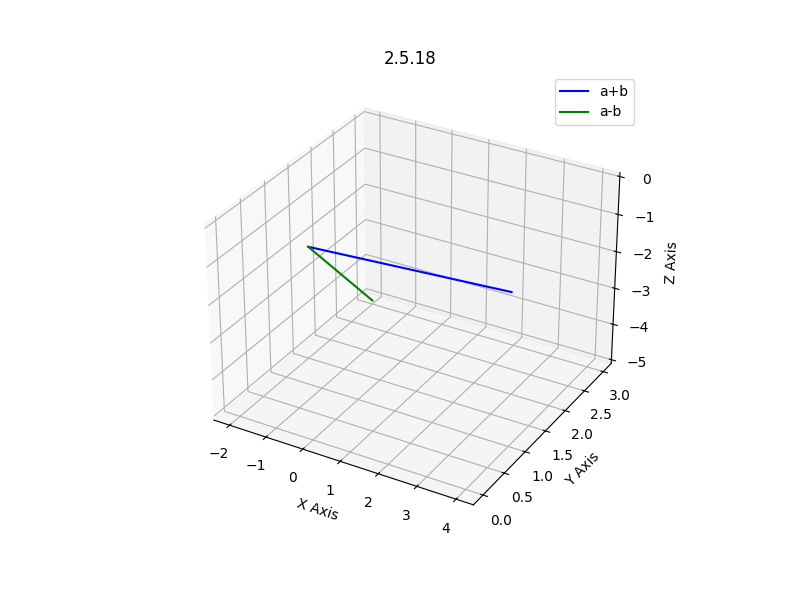
\includegraphics{figs/plot.png}
    \caption*{}
    \label{fig:plot}
\end{figure}
\end{document}
